\section{Résultats}

\begin{minipage}{\textwidth}
    \begin{wrapfigure}{R}{0.55\textwidth}
        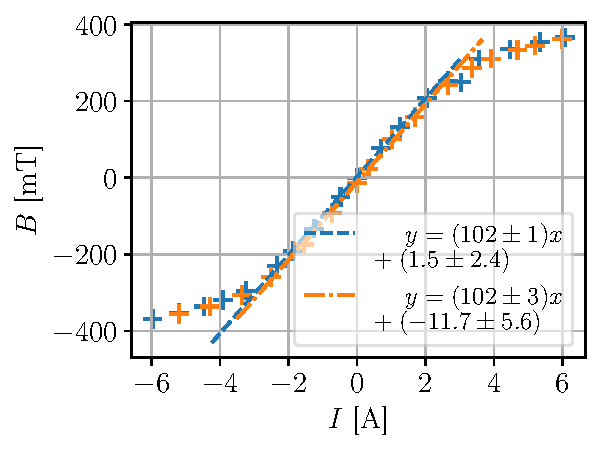
\includegraphics[width=\linewidth]{figures/calibration.pdf}
        \caption{Variation de l'amplitude du champ magnétique en fonction du courant sur un cycle \(I_\textrm{max} \rightarrow 0 \rightarrow -I_\textrm{max} \rightarrow 0 \rightarrow I_\textrm{max}\).}
        \label{fig:callibration}
    \end{wrapfigure}

    \paragraph*{Étalonnage du champ d'induction}
    La \autoref{fig:callibration} montre comment varie le champ magnétique en fonction du courant. Ici, \(I_\textrm{max} = 6\) \si{\ampere}. Par souci de clarté, les erreurs sur les mesures ne sont pas affichées dans cette figure et sont de l'ordre de 2\%, dont les calculs sont détaillés dans \autoref{sec:erreurs}. Les points bleus correspondent à la partie descendante du cycle et les points oranges à la partie montante. Deux fit linéaire on été réalisés sur la partie linéaire (entre -3 \si{\ampere} et 3 \si{\ampere}), 1 pour chaque sens, et mettent en évidence une légère hystérèse, puisque les deux droites sont décalées, d'ordonnée à l'origine \(\beta_1 = (1.5 \pm 1.6)\) pour la partie \(I_\textrm{max} \rightarrow 0 \rightarrow -I_\textrm{max}\) contre \(\beta_2 = (-11.7 \pm 2.4)\) pour la partie \(-I_\textrm{max} \rightarrow 0 \rightarrow I_\textrm{max}\).

\end{minipage}

\paragraph*{Tensions résiduelles}
Le \autoref{tab:tension_residuelle} montre les tensions résiduelle dans deux échantillons d'InP dopés au Si d'épaisseurs 1 \si{\micro\meter} et 2 \si{\micro\meter}. Les mesures ont été réalisées avec un champ magnétique de 0 \si{\milli\tesla} et un courant (\(I = 1.002 \pm 0.001\)) \si{\milli\ampere} pour le premier échantillon \(I = (1.001 \pm 0.001)\) \si{\milli\ampere} pour le deuxième échantillon. La configuration \(I_{24}U_{13}\) donnant la plus faible tension résiduelle ce sera celle conservée pour le reste des mesures. La différence de 0.02 \si{\milli \volt} entre \(I_{24}U_{13}\) et \(I_{42}U_{31}\) pour l'échantillon de 2 \si{\micro\meter} est considérée négligeable.

\begin{table}[h]
    \centering
    \begin{tabulary}{\textwidth}{C C C C}
        \toprule
        Configuration \si{\micro\meter} & Tension (\(a = 1\) \si{\micro\meter}) [\si{\milli\volt}] & Tension (\(a = 2\) \si{\micro\meter}) [\si{\milli\volt}] \\
        \midrule
        \(I_{13}U_{24}\) & \(68.74 \pm 0.01\) & \(27.02 \pm 0.01\) \\
        \(I_{31}U_{42}\) & \(68.69 \pm 0.01\) & \(27.12 \pm 0.01\) \\
        \(I_{24}U_{13}\) & \(39.93 \pm 0.01\) & \(24.78 \pm 0.01\) \\
        \(I_{42}U_{31}\) & \(40.12 \pm 0.01\) & \(24.76 \pm 0.01\) \\
        \bottomrule
    \end{tabulary}
    \caption{Tension résiduelle pour différentes configuration et 2 épaisseurs de l'échantillon InP dopés au Si}
    \label{tab:tension_residuelle}
\end{table}

\paragraph*{Détermination de la constante de Hall}
Afin de déterminer la constante de Hall des deux échantillon d'InP dopés au Si, un champ magnétique constant de \(B = (348 \pm 6)\) \si{\milli\tesla} et (\(B = 383 \pm 7\)) \si{\milli\tesla} à été appliqués aux échantillons de 1 \si{\micro\meter} et 2 \si{\micro\meter} respectivement. Les \autoref{fig:inpV(I)} et \autoref{fig:inpV(B)} montrent la variation de la tension de Hall en fonction du courant dans l'échantillon et du champ magnétique respectivement. Les coefficients des regressions linéaires permettent de déterminer à l'aide de l'\autoref{eq:R_H} les valeurs du coefficient de Hall \(R_H\) et avec l'\autoref{eq:N} la densité de porteurs de charge \(N\). Les résultats sont reportés dans le \autoref{tab:RH_N}.

\begin{figure}[h]
    \centering
    \begin{subfigure}{0.5\textwidth}
        \centering
        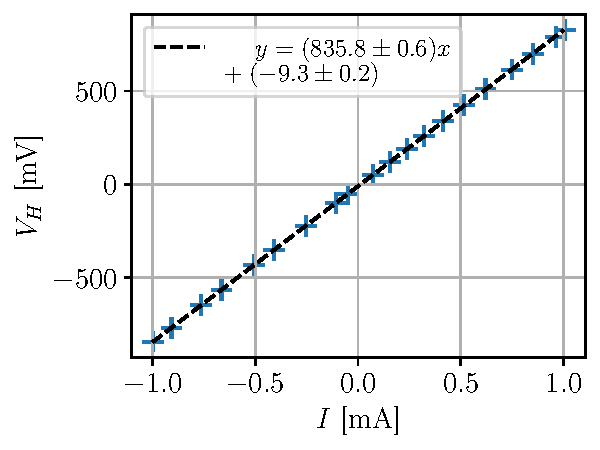
\includegraphics[width=\textwidth]{figures/U(I),InP1micro.pdf}
        \caption{}
    \end{subfigure}%
    \begin{subfigure}{0.5\textwidth}
        \centering
        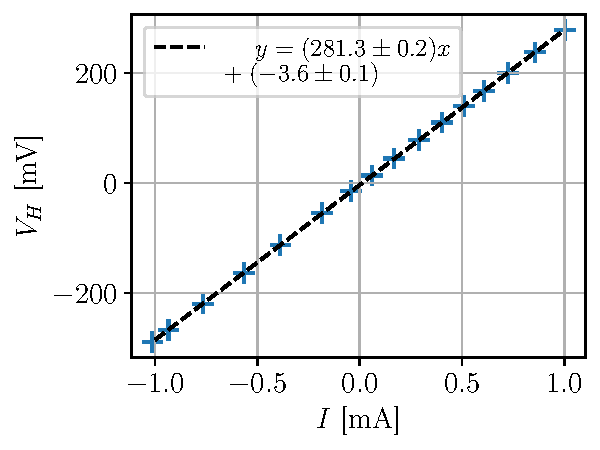
\includegraphics[width=\textwidth]{figures/U(I),InP2micro.pdf}
        \caption{}
    \end{subfigure}
    \caption{Tension en fonction de l'intensité pour l'échantillon InP d'épaisseur (a) 1 \si{\micro\meter} (b) 2 \si{\micro\meter}}
    \label{fig:inpV(I)}
\end{figure}

\begin{table}[h]
    \centering
    \begin{tabulary}{\textwidth}{C C C C C}
        \toprule
        Échantillon & \(R_H^B\) [\si{\meter\cubed\per\coulomb}] & \(R_H^I\) [\si{\meter\cubed\per\coulomb}] & \(N^B\) [\si{\per\meter\cubed}] & \(N^I\) [\si{\per\meter\cubed}] \\
        \midrule
        1 \si{\micro\meter} & \((-2.40 \pm 0.05) \cdot 10^{-3}\) & \((-2.24 \pm 0.02) \cdot 10^{-3}\) & \((2.60 \pm 0.05) \cdot 10^{21}\) & \((2.79 \pm 0.03) \cdot 10^{21}\) \\
        2 \si{\micro\meter} & \((-1.47 \pm 0.03) \cdot 10^{-3}\) & \((-1.62 \pm 0.01) \cdot 10^{-3}\) & \((4.25 \pm 0.08) \cdot 10^{21}\) & \((3.84 \pm 0.02) \cdot 10^{21}\) \\
        \bottomrule
    \end{tabulary}
    \caption{Constante de Hall \(R_H\) et densité de porteurs de charges \(N\) pour les différents échantillons}
    \label{tab:RH_N}
\end{table}

\paragraph*{Echantillons à 5 contacts}

La deuxième partie de l'expérience consiste à trouver ces valeurs \(R_H\) et \(N\) pour 3 échantillons à 5 contacts. Pour ce faire la même méthode a été utilisée de mesurer la tension de Hall \(V_H\) en fonction du champ magnétique \(B\) à \(I\) constant et en fonction du courant \(I\) à \(B\) constant. Les résultat de la première méthode sont visibles dans la \autoref{fig:5branch_B} pour les régressions linéaires et dans le \autoref{tab:5branch_B} avec les valeurs obtenues et leurs incertitudes. La valeur de \(R_H\) est obtenue à partir de l'épaisseur \(a\) de l'intensité constante \(I\) et de la valeur du coefficient \(\alpha_I\) obtenu par régression linéaire sur les mesures de \(V_H\) en fonction de \(B\). La valeur de \(N\) est elle calculée à partir de \(R_H\) et de la valeur de la charge élémentaire des électrons \(q_- = -1.602176634\times10^{-19}\) \si{\coulomb} qui est considérée sans incertitude ici puisqu'il s'agit d'une valeur tabulée issue de la littérature. Il est nécessaire d'utilisé \(q_-\) négatif ici car il est connu que \(R_H\) a le même signe que la charge des porteurs de charge et toutes les valeurs de \(R_H\) obtenues sont négatives.

Les résultats de la deuxième méthode à \(B\) constants sont visibles dans la \autoref{fig:5branch_I} en \autoref{sec:supp} avec les valeurs dans le \autoref{tab:5branch_I} et résultent du même procédé d'analyse des mesures.

\begin{figure}[h]
    \centering
    \begin{subfigure}{0.33\textwidth}
        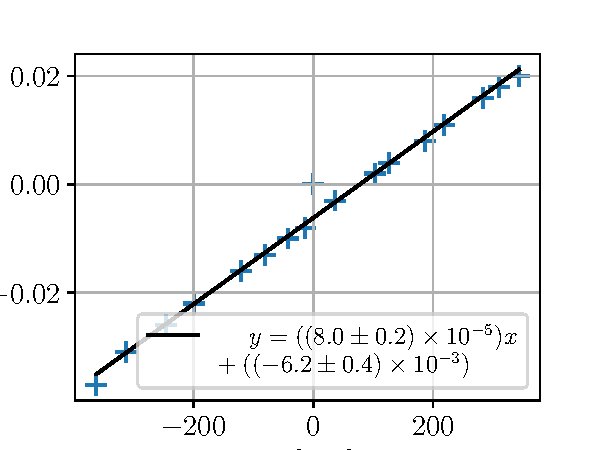
\includegraphics[width=\linewidth]{figures/Ag_B.pdf}
        \caption{}
        \label{fig:Ag_B}
    \end{subfigure}%
    \begin{subfigure}{0.33\textwidth}
        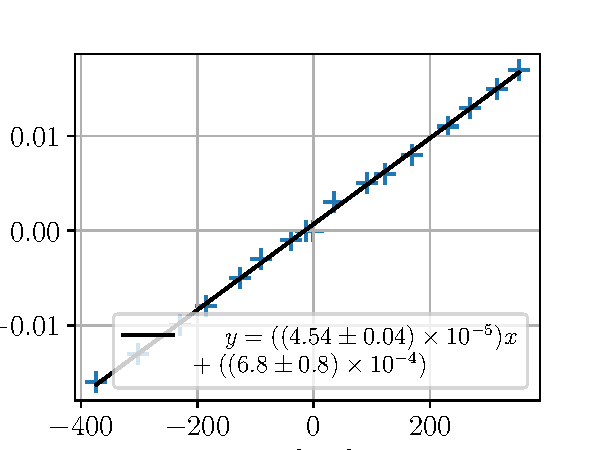
\includegraphics[width=\linewidth]{figures/Cu_B.pdf}
        \caption{}
        \label{fig:Cu_B}
    \end{subfigure}%
    \begin{subfigure}{0.33\textwidth}
        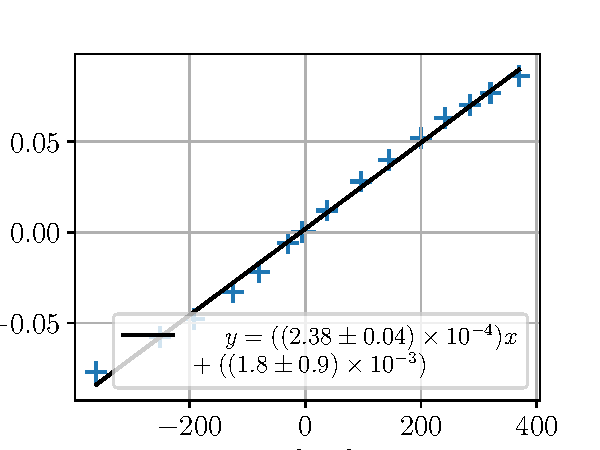
\includegraphics[width=\linewidth]{figures/Bi_B.pdf}
        \caption{}
        \label{fig:Bi_B}
    \end{subfigure}
    \caption{Régressions de \(V_H\) en fonction de \(B\) à \(I\) constant pour (a) Ag, (b) Cu et (c) Bi}
    \label{fig:5branch_B}
\end{figure}

\begin{table}[h]
    \centering
    \begin{tabulary}{\textwidth}{C C C C}
        \toprule
        échantillon & \(\alpha_B = \frac{V_H}{B}\) & \(R_H = -\frac{\alpha_B a}{I}\) & N [\si{\per \cubic \meter}] \\
        \midrule
        Ag & \((8.0 \pm 0.2) \times 10^{-5}\) & \((-7.7 \pm 0.2) \times 10^{-11}\) & \((8.1 \pm 0.2) \times 10^{28}\) \\
        Cu & \((4.54 \pm 0.04) \times 10^{-5}\) & \((-3.65 \pm 0.03) \times 10^{-11}\) & \((1.71 \pm 0.02) \times 10^{29}\) \\
        Bi & \((2.38 \pm 0.04) \times 10^{-4}\) & \((-3.62 \pm 0.07) \times 10^{-7}\) & \((1.72 \pm 0.03) \times 10^{25}\) \\
        \bottomrule
    \end{tabulary}
    \caption{Valeurs de \(R_H\) et \(N\) obtenues pour les échantillons à 5 branchements à \(I\) constant}
    \label{tab:5branch_B}
\end{table}
